\section{Impressum}
\subsection{Projektteam}
Das Projektteam besteht aus folgenden Schülern:\\

\begin{table}[H]
  \begin{center}
    \begin{tabular}{|p{0.2\textwidth}|p{0.55\textwidth}|p{0.25\textwidth}|}
      \hline
      \textbf{Name}  & \textbf{Aufgabenstellung}                                                                                                                                                                                                                                & \textbf{Bild}                                                                           \\
      \hline
      Paul Hartmann  & Paul übernahm die Projektleitung und war für die Kommunikation mit dem Partnerunternehmen zuständig. Er recherchierte zu Varianten zur Lagerung von Fahrrädern und führte die Nutzwertanalyse und Umfrage aus. Paul entwickelte die Mobile-App.          & \begin{minipage}{.3\textwidth} 
\includegraphics{images/paulhartmann.jpg} \end{minipage} \\
      \hline
      Joshua Lung    & Joshua recherchierte zu Varianten zur Lagerung von Fahrrädern, führte die Nutzwertanalyse aus, erstellte Fragen der Umfrage und konzeptionierte das Rondell-Modell. Er baute den Prototyp des Turmes und übernahm die Softwareentwicklung der Steuerung. & \begin{minipage}{.3\textwidth}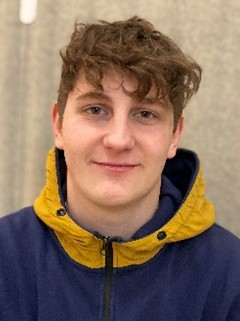
\includegraphics{images/joshualung.jpg} \end{minipage}    \\
      \hline
      Lukas Madlener & Lukas erstellte Skizzen für verschiedene automatisierte Arten zur Lagerung von Fahrrädern und konzeptionierte das Hochregallager. Er testete NFC-Technologien mit einer Mobile-App.                                                                      & \begin{minipage}{.3\textwidth}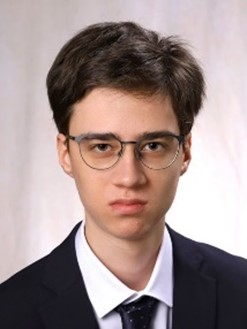
\includegraphics{images/lukasmadlener.jpg} \end{minipage} \\
    \end{tabular}
    \caption{Projektteam}
    \label{tab:projektteam}
  \end{center}
\end{table}

\subsection{Projektbetreuer der Schule}
\begin{table}[H]
  \begin{center}
    \begin{tabular}{|p{0.2\textwidth}|p{0.55\textwidth}|p{0.25\textwidth}|}
      \hline
      \textbf{Name}  & \textbf{Rolle}                                                                                                                                                                                                                                & \textbf{Bild}                                                                           \\
      \hline
      Prof. MMag. Hämmerle Günter & Günter Hämmerle initiierte das Projekt mit dem Partnerunternehmen LTW Intralogistics und war bei allen Besprechungen mit dem Partnerunternehmen dabei. Er unterstützte das Team in allen Projektphasen, besonders bei der Analyse der Kosten und der Dokumentation der Diplomarbeit.          & \begin{minipage}{.3\textwidth} 
\includegraphics{images/günterhämmerle.jpg} \end{minipage} \\
      \hline
      Prof. Mag. Riedmann Andreas & Andreas Riedmann unterstützte das Team bei der Auswahl der Technologien zur Softwareentwicklung und bei der Dokumentation der Diplomarbeit. & \begin{minipage}{.3\textwidth}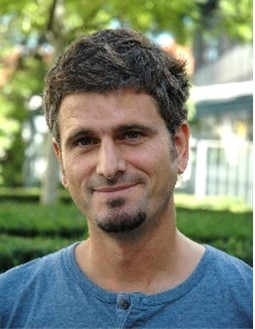
\includegraphics{images/andreasriedmann.jpg} \end{minipage}    \\
    \end{tabular}
    \caption{Projektbetreuer}
    \label{tab:projektbetreuer}
  \end{center}
\end{table}

\subsection{Projektbetreuer vom Partnerunternehmen}
Johannes Schwartze war der Betreuer der Diplomarbeit vonseiten des Partnerunternehmens LTW Intralogistics. Er war der Ansprechpartner bei Fragen und gab neue Aufgabestellungen und Feedback. Beim Partnerunternehmen gab es mehrere Besprechungen, wo die Fortschritte präsentiert und diskutiert wurden.  \\